\documentclass[10pt, onecolumn] {IEEEtran}

\usepackage[utf8x]{inputenc}
\usepackage[frenchb]{babel}
\usepackage[T1]{fontenc}
\usepackage{lmodern}
\usepackage{fullpage}
\usepackage{graphicx}
\usepackage{epstopdf}
\usepackage{caption}
\usepackage{subcaption}
\usepackage{multirow}
\usepackage{hyperref}

% Math symbols
\usepackage{amsmath}
\usepackage{amssymb}
\usepackage{amsthm}
\usepackage{mathtools}

% Numbers and units
\usepackage[squaren, Gray]{SIunits}
\usepackage{sistyle}
\usepackage[autolanguage]{numprint}
%\usepackage{numprint}
\newcommand\si[2]{\numprint[#2]{#1}}
\newcommand\np[1]{\numprint{#1}}

\DeclareMathOperator{\newdiff}{d} % use \dif instead
\newcommand{\dif}{\newdiff\!}
\newcommand{\fpart}[2]{\frac{\partial #1}{\partial #2}}
\newcommand{\ffpart}[2]{\frac{\partial^2 #1}{\partial #2^2}}
\newcommand{\fdpart}[3]{\frac{\partial^2 #1}{\partial #2\partial #3}}
\newcommand{\fdif}[2]{\frac{\dif #1}{\dif #2}}
\newcommand{\ffdif}[2]{\frac{\dif^2 #1}{\dif #2^2}}
\newcommand{\constant}{\ensuremath{\mathrm{cst}}}

\newcommand{\bigoh}{\mathcal{O}}

% cfr http://en.wikibooks.org/wiki/LaTeX/Colors
\usepackage{color}
\usepackage[usenames,dvipsnames,svgnames,table]{xcolor}
\definecolor{dkgreen}{rgb}{0.25,0.7,0.35}
\definecolor{dkred}{rgb}{0.7,0,0}

\usepackage{listings}
\lstset{
  numbers=left,
  numberstyle=\tiny\color{gray},
  basicstyle=\rm\small\ttfamily,
  keywordstyle=\bfseries\color{dkred},
  frame=single,
  commentstyle=\color{gray}=small,
  stringstyle=\color{dkgreen},
  %backgroundcolor=\color{gray!10},
  %tabsize=2,
  rulecolor=\color{black!30},
  %title=\lstname,
  breaklines=true,
  framextopmargin=2pt,
  framexbottommargin=2pt,
  extendedchars=true,
  inputencoding=utf8x
}

\lstset{language={C}}

\title{INGI1113\\
Minix3 Projet 2013-2014\\
Rapport : Groupe 23}

\author{Jos Zigabe  \and Mehdi Dumoulin}

\begin{document}

\maketitle
\tableofcontents
\newpage

\section{introduction au projet}

Dans le cadre du cours de \og Systèmes informatiques 2 \fg, il nous a été demandé pour le troisième projet de modifier l'OS Minix3. Dans un premier temps afin de se familiariser avec l'architecture de Minix, on a dû implémenter un appel système \texttt{get\_pidinfo} à ajouter au code source et ensuite on a dû implémenter un nouveau mode d'accès des fichiers système pour MFS qui permettra de les crypter.      

\subsection{Description de notre architecture}

Pour la première phase, on donc dû implémenter l'appel système \texttt{getpidinfo} grâce à la fonction : \texttt{get\_pidinfo(struct pid\_s *pids)} avec en paramètre une structure censé contenir l'ID du processus parent et de sont fils. La fonctionnalité de cette fonction est très simple elle doit juste récupérer les ID du parent et du fils, en lançant un appel système à  \texttt{getpidinfo}.\\

\subsubsection{Descriptions des fichiers ajouté et modifiers }

Afin de rajouter notre appel nous sommes passé par deux étapes : la première consistant à créer un gestionnaire d'appel-système qui est la fonction appelé en réponse à l'appel de \texttt{getpidinfo} et une librairie utilisateur qui assemble les paramètre pour l'appel système et qui appel le gestionnaire de notre appel  \texttt{getpidinfo}.\\

\begin{itemize}
\item \textbf{Gestionnaire de système d'appel} : Premièrement il nous a fallu localiser le serveur adéquat qui dans notre cas est pm \og process manager \fg qui s'occupe des appels systèmes relative à la gestion de processus ou encore à examiner les propriétés des processus ce qui est notre cas. Ensuite chaque serveur possède 2 fichiers : \\ \texttt{table.c} qui contient la définition d'un tableau de pointeurs de fonction indexé par le numéro du système d'appel avec donc à chaque ligne l'adresse de la fonction du gestionnaire d'appel. Nous avons donc dû rajouter dans ce tableau \texttt{call\_vec} la fonction du gestionnaire d'appel de \texttt{do\_getpidinfo,	\slash* 31 = pidinfo	*\slash} indexé au numéro de son appel système. Il y a ensuite le fichier  \texttt{proto.h} qui contient les prototypes de tous les fonctions des gestionnaires d'appel système, dans lequel nous avons dû également y inclure notre prototype \texttt{\_PROTOTYPE( int do\_getpidinfo, (void)					)}. Et on a également implémenté la fonction  \texttt{do\_getpidinfo} dans le fichier /src/servers/pm/misc.c.\\

\item \textbf{Fonction de librairie d'utilisateur} : Tout d'abord, nous avons dû modifier le fichier /src/include/minix/callnr.h afin d'attribuer un numéro à l'appel système de la fonction du gestionnaire \texttt{\#define GETPIDINFO 31}. Ensuite nous avons implémenté la fonction de librairie d'utilisateur \texttt{\_getpidinfo.c} dans le dossier /src/lib/libc/posix/ afin que l'appel puisse être utilisé par n'importe quel programme C.  \\
\end{itemize}

Pour finir nous avons implémenté la structure \texttt{pid\_s} que nous avons placé dans le fichier /src/include/sys/pid\_s.h, fichier dans lequel on a mis le prototype de la fonction : \texttt{\_PROTOTYPE( int getpidinfo, (struct pid\_s *pids)            )}. Ensuite nous avons ajouté le fichier /src/lib/libc/syscall/getpidinfo.S qui permet de convertir \texttt{getpidinfo} en  \texttt{\_getpidinfo} afin que l'appel à \texttt{getpidinfo(struct pid\_s *pids);} soit possible. 

\newpage
\section{Projet principal}

Comme demandé, nous avons fait une copie du fichier /src/commands/mount/mount.c que nous avons modifié et placé dans le dossier test pour pouvoir l'utiliser pour monter des disques cryté. Pour ce faire, une nouvelle comparaison a été ajoutée dans le \texttt{case} afin de vérifier si \texttt{-e} a été saisi par l'utilisateur. Si il a été saisi, un \texttt{OR Logique} est appliqué sur la variable \texttt{mountflags} pour que l'on puisse retrouver si cette option a été activée dans d'autres fichiers de Minix. Cette variable sert aussi notamment a savoir si le disque est monter en mode lecture seule ou non.

Lors de la réalisation de notre projet nous avons dû faire face à quelques problèmes. Premièrement on s'est posé des questions concernant la gestion de clé : car on avait le choix entre faire confiance à l'utilisateur et lui laisser entrer la clé ou attribuer une clé à chaque \texttt{FS} que l'on stockerait dans chaque \texttt{superblock} que chaque \texttt{FS} possède afin d'y stocker des informations spécifiques à chaque \texttt{FS}.  Ensuite, il a du choisir entre crypter le buffer dans le \texttt{MFS} ou dans le \texttt{VFS} car c'est deux solutions solutions était toutes deux correctes mais l'une entre elle avait un avantage sur l'autre.\\   

\subsection{Architecture}

Avant d'implémenter notre solution nous avions tout d'abord compris que le \texttt{VFS} était une sorte de système de fichier abstrait qui était au dessus des autres \texttt{FS}. Il offre ainsi une interface d'accès commune à tous les autres système de fichier qui cache de ce fait les propriété de chaque \texttt{FS} dans le \texttt{VFS}. 

\begin{figure}[h]
\begin{center}
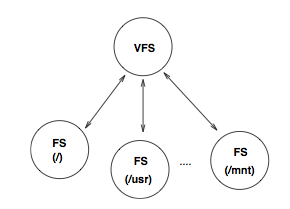
\includegraphics [scale=0.5] {figures/VFS-FS.png} 
\caption{Hiérarchie entre \texttt{FS}}
\label{default}
\end{center}
\end{figure}
     
Le \texttt{VFS} accède à l'implémentation des \texttt{FS} à travers des pointeurs de fonctions et communique avec eux grâce aux \texttt{message}. \\

Pour que notre système de cryptage/décryptage fonctionne avec tous les \texttt{FS}, nous avons décidé de l'implémenter dans \texttt{VFS}. En effet, nous avons mis notre code dans le fichier \texttt{read.c} de \texttt{VFS} dans la méthode \texttt{read\_write}. Cette méthode fait appel à une requête pour pouvoir appeler le  \texttt{FS} correspondant au disque monté et lire la partie du fichier voulue. Cette méthode permettant à la fois de lire et d'écrire dans un fichier, le cryptage/décryptage se situe à différents endroit :

\begin{itemize}
\item Lecture dans un fichier : ici il faut intercepter le buffer, après que le \texttt{FS} ai fait son boulot, grâce à \texttt{sys\_datacopy}, ensuite il suffit de le décrypter et de renvoyer cette nouvelle version au processus utilisateur.
\item Ecrite dans un fichier : dans ce cas-ci, il faut intercepter le buffer qui est passé au \texttt{FS} et qui contient le contenu de ce que l'on veut écrire dans le fichier pour pouvoir le crypter. Pour ce faire, on utilise la fonction \texttt{sys\_datacopy}, qui permet de récuperer les données contenu dans l'espace utilsateur, et on applique notre méthode de cryptage sur ce contenu. Nous discuterons plus loin de la méthode utilisé pour le cryptage/décryptage.
\end{itemize}

\subsection{Gestion de la clé}

Nous avons choisi de demander la clé à l'utilisateur et non d'enregistrer la clé dans le \texttt{superblock} car la modification de ce dernier est fort complexe. Ainsi dans la fonction \texttt{mount} du fichier \texttt{/src/lib/libc/other/\_mount.c} on teste d'abord le \texttt{mountflag} et si la valeur contenue est \texttt{MS\_CRYPT}, on alloue de l'espace pour la clé de cryptage que l'on demande via un \texttt{scanf}. Ensuite on ne savait pas trop comment intégrer cette clé dans le \texttt{message} afin que le \texttt{VFS} puisse l'utiliser, étant donnée qu'il n'y avait plus de sous-variable dans le structure \texttt{message} pour la contenir. Face à ce problème nous avons donc décidé d'ajouter une sous-variable \texttt{char *m1p4} de la structure \texttt{mess\_1} défini dans le fichier \texttt{/src/include/minix/ipc.h}. Et suite à cette modification de la structure \texttt{mess\_1}, on a pu transférer la clé provenant de l'espace utilisateur au \texttt{VFS}. Enfin étant donnée que l'on était incapable de manipuler le \texttt{superblock}, on a décider pour la suite d'enregistrer la clé dans la structure \texttt{vmnt} qui stocke les informations relative à la partition attachée. Ainsi nous avons modifié cette structure en ajoutant une nouvelle sous-variable afin de contenir la clé du cryptage.     





\end{document}